\item \textbf{{[}ALVL/9597/2019/P1/Q3{]} }

A program is to be written to represent and implement a linked list
of nodes. Each node contains a string data value and a pointer. The
pointers link the data items in alphabetical order. 

The unused nodes are linked as shown below. The first unused node
is the position where the next new data item is to be stored. 
\begin{center}
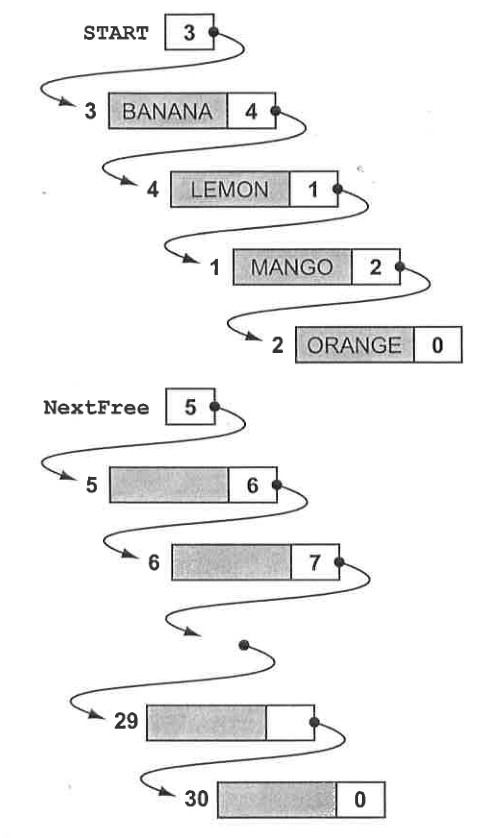
\includegraphics[width=0.25\paperwidth]{C:/Users/Admin/Desktop/Github/question_bank/LyX/static/img/9597-ALVL-2014-P1-Q3}
\par\end{center}

The diagram shows the linked list with: 
\begin{itemize}
\item the items MANGO, ORANGE, BANANA and LEMON (added in that order). 
\item the unused nodes linked together.
\end{itemize}
Each node is implemented as an instance of the class\texttt{ ListNode}.
The class \texttt{ListNode} has the following properties: 
\begin{center}
\begin{tabular}{|l|c|l|}
\hline 
\multicolumn{3}{|c|}{Class\texttt{: ListNode}}\tabularnewline
\hline 
\multicolumn{3}{|c|}{Properties}\tabularnewline
\hline 
\texttt{\hspace{0.01\columnwidth}}Identifier & \texttt{\hspace{0.01\columnwidth}}Data Type & \texttt{\hspace{0.01\columnwidth}}Description\tabularnewline
\hline 
\texttt{DataValue} & \texttt{STRING} & The node data\tabularnewline
\hline 
\texttt{PointerValue} & \texttt{INTEGER} & The node pointer\tabularnewline
\hline 
\end{tabular}
\par\end{center}

A linked list is implemented as an instance of the class \texttt{LinkedList}.
The class \texttt{LinkedList} has the following properties and methods: 
\begin{center}
\begin{tabular}{|l|c|>{\raggedright}p{0.25\columnwidth}|}
\hline 
\multicolumn{3}{|c|}{Class\texttt{: LinkedList}}\tabularnewline
\hline 
\multicolumn{3}{|c|}{Properties}\tabularnewline
\hline 
\texttt{\hspace{0.01\columnwidth}}Identifier & \texttt{\hspace{0.01\columnwidth}}Data Type & \texttt{\hspace{0.01\columnwidth}}Description\tabularnewline
\hline 
\texttt{Node} & \texttt{ARRAY{[}30{]} OF ListNode} & The linked list data structure --- data values and pointers.The array
index starts at 1.For testing purposes the dataset has a maximum of
30 items.\tabularnewline
\hline 
\texttt{Start} & \texttt{INTEGER} & Index position of the node at the start of the linked list\tabularnewline
\hline 
\texttt{NextFree} & \texttt{INTEGER} & Index position of the next unused node \tabularnewline
\hline 
\multicolumn{3}{|l|}{Methods}\tabularnewline
\hline 
\texttt{\hspace{0.01\columnwidth}}Identifier &  & \texttt{\hspace{0.01\columnwidth}}Description\tabularnewline
\hline 
\texttt{Initialise} & \texttt{PROCEDURE} & Sets all the node data values to \textquoteleft empty string\textquoteright .

Set pointers to indicate all nodes are unused and linked.

lnitialise values for \texttt{Start} and \texttt{NextFree}.\tabularnewline
\hline 
\texttt{AddNode} & \texttt{PROCEDURE} & Add a new data item to the linked list.\tabularnewline
\hline 
\texttt{Traversal} & \texttt{PROCEDURE} & Display the data items in order.\tabularnewline
\hline 
\texttt{ReverseTraversal} & \texttt{PROCEDURE} & Display the data items in reverse order.\tabularnewline
\hline 
\texttt{DisplayLinkedList} & \texttt{PROCEDURE} & Display the current state of pointers and the array contents.\tabularnewline
\hline 
\texttt{IsEmpty} & \texttt{FUNCTION RETURNS BOOLEAN} & Tests for empty linked list.\tabularnewline
\hline 
\texttt{IsFull} & \texttt{FUNCTION RETURNS BOOLEAN} & Tests for no unused nodes.\tabularnewline
\hline 
\end{tabular}
\par\end{center}

\subsubsection*{Task 3.1}

Write program code that repeatedly:
\begin{itemize}
\item displays a menu with the following choices: 
\begin{enumerate}
\item[1.]  Add an item 
\item[2.]  Traverse the linked list of used nodes and output the data values 
\item[3.]  Output all pointers and data values 
\item[4.]  Exit 
\end{enumerate}
\item calls an appropriate procedure depending on the user's choice. 
\end{itemize}

\subsubsection*{Evidence 8}

Program code for Task 3.1.\hfill{} {[}5{]}

\subsubsection*{Task 3.2}

Write program code for the classes \texttt{ListNode} and \texttt{LinkedList}
including the \texttt{IsEmpty} method. The code should follow the
specification given. 

Do not attempt to write the methods \texttt{AddNode}, \texttt{Traversal},
\texttt{ReverseTraversal} or \texttt{IsFull} at this stage. 

\subsubsection*{Evidence 9}

Program code for the \texttt{ListNode} and \texttt{LinkedList} classes
(Task 3.2).\hfill{} {[}12{]}

\subsubsection*{Task 3.3}

Write code to create a \texttt{LinkedList} object in the main program.

Run the program and select menu choice 3 to confirm the initial values
of the pointers and data values when the linked list is empty. {[}10{]}

\subsubsection*{Evidence 10}

Screenshot confirming all values after initialisation of the \texttt{LinkedList}
object (Task 3.3). 

\hfill{} {[}3{]}

\subsubsection*{Task 3.4}

Consider the \texttt{AddNode} method. The following algorithm will
add a new data item to the linked list. 

The algorithm uses the variables below:
\begin{center}
\begin{tabular}{|l|c|>{\raggedright}p{0.25\columnwidth}|}
\hline 
\texttt{\hspace{0.01\columnwidth}}Identifier & \texttt{\hspace{0.01\columnwidth}}Data Type & \texttt{\hspace{0.01\columnwidth}}Description\tabularnewline
\hline 
\texttt{NewItem} & \texttt{STRING} & New data item input by the user\tabularnewline
\hline 
\texttt{Found} & \texttt{BOOLEAN} & Flags to \texttt{TRUE} when the position at which to insert the new
item has been found\tabularnewline
\hline 
\texttt{Current} & \texttt{INTEGER} & Current array index position during list traversal\tabularnewline
\hline 
\texttt{Previous} & \texttt{INTEGER} & Previous array index position during list traversal\tabularnewline
\hline 
\texttt{Temp} & \texttt{INTEGER} & Temporary storage of pointer value\tabularnewline
\hline 
\end{tabular}
\par\end{center}

\noindent\fbox{\begin{minipage}[t]{1\columnwidth - 2\fboxsep - 2\fboxrule}%
\texttt{PROCEDURE AddNode }

\texttt{\qquad{}INPUT NewItem }

\texttt{\qquad{}Node{[}NextFree{]}.DataValue <\textemdash{} NewItem }

\texttt{\qquad{}IF Start = 0 }

\texttt{\qquad{}\qquad{}THEN }

\texttt{\qquad{}\qquad{}Start <\textemdash{} NextFree }

\texttt{\qquad{}\qquad{}Temp <\textemdash{} Node{[}NextFree{]}.PointerValue }

\texttt{\qquad{}\qquad{}Node{[}NextFree{]}.PointerValue <\textemdash{}
0 }

\texttt{\qquad{}\qquad{}NextFree <\textemdash{} Temp }

\texttt{\qquad{}ELSE }

\texttt{\qquad{}\qquad{}// traverse the list - starting at Start
to find }

\texttt{\qquad{}\qquad{}// the position at which to insert the new
item }

\texttt{\qquad{}\qquad{}Temp <\textemdash{} Node{[}NextFree{]}.PointerValue }

\texttt{\qquad{}\qquad{}IF NewItem < Node{[}Start{]}.DataValue }

\texttt{\qquad{}\qquad{}\qquad{}THEN }

\texttt{\qquad{}\qquad{}\qquad{}\qquad{}// new item will become
the start of the list }

\texttt{\qquad{}\qquad{}\qquad{}\qquad{}Node{[}NextFree{]}.PointerValue
<\textemdash{} Start }

\texttt{\qquad{}\qquad{}\qquad{}\qquad{}Start <\textemdash{} NextFree }

\texttt{\qquad{}\qquad{}\qquad{}\qquad{}NextFree <\textemdash{}
Temp }

\texttt{\qquad{}\qquad{}\qquad{}ELSE }

\texttt{\qquad{}\qquad{}\qquad{}\qquad{}// the new item is not
at the start of the list }

\texttt{\qquad{}\qquad{}\qquad{}\qquad{}Previous <\textemdash{}
0 }

\texttt{\qquad{}\qquad{}\qquad{}\qquad{}Current <\textemdash{}
Start }

\texttt{\qquad{}\qquad{}\qquad{}\qquad{}Found <\textemdash{} False }

\texttt{\qquad{}\qquad{}\qquad{}\qquad{}REPEAT }

\texttt{\qquad{}\qquad{}\qquad{}\qquad{}\qquad{}IF NewItem <=
Node{[}Current{]}.DataValue }

\texttt{\qquad{}\qquad{}\qquad{}\qquad{}\qquad{}\qquad{}THEN }

\texttt{\qquad{}\qquad{}\qquad{}\qquad{}\qquad{}\qquad{}\qquad{}Node{[}Previous{]}.PointerValue
<\textemdash{} NextFree }

\texttt{\qquad{}\qquad{}\qquad{}\qquad{}\qquad{}\qquad{}\qquad{}Node{[}NextFree{]}.PointerValue
<\textemdash{} Current }

\texttt{\qquad{}\qquad{}\qquad{}\qquad{}\qquad{}\qquad{}\qquad{}NextFree
<\textemdash{} Temp }

\texttt{\qquad{}\qquad{}\qquad{}\qquad{}\qquad{}\qquad{}\qquad{}Found
<\textemdash{} True }

\texttt{\qquad{}\qquad{}\qquad{}\qquad{}\qquad{}\qquad{}ELSE }

\texttt{\qquad{}\qquad{}\qquad{}\qquad{}\qquad{}\qquad{}\qquad{}//
move on to the next node }

\texttt{\qquad{}\qquad{}\qquad{}\qquad{}\qquad{}\qquad{}\qquad{}Previous
<\textemdash{} Current }

\texttt{\qquad{}\qquad{}\qquad{}\qquad{}\qquad{}\qquad{}\qquad{}Current
<\textemdash{} Node{[}Current{]}.PointerValue }

\texttt{\qquad{}\qquad{}\qquad{}\qquad{}\qquad{}ENDIF }

\texttt{\qquad{}\qquad{}\qquad{}\qquad{}UNTIL Found = True OR
Current = 0 }

\texttt{\qquad{}\qquad{}\qquad{}\qquad{}IF Current <\textemdash{}
0 }

\texttt{\qquad{}\qquad{}\qquad{}\qquad{}\qquad{}THEN }

\texttt{\qquad{}\qquad{}\qquad{}\qquad{}\qquad{}\qquad{}Node{[}Previous{]}.PointerValue
<\textemdash{} NextFree }

\texttt{\qquad{}\qquad{}\qquad{}\qquad{}\qquad{}\qquad{}Node{[}NextFree{]}.PointerValue
<\textemdash{} 0 }

\texttt{\qquad{}\qquad{}\qquad{}\qquad{}\qquad{}\qquad{}NextFree
<\textemdash{} Temp }

\texttt{\qquad{}\qquad{}\qquad{}\qquad{}ENDIF }

\texttt{\qquad{}\qquad{}ENDIF }

\texttt{\qquad{}ENDIF }

\texttt{ENDPROCEDURE }

Note: The above pseudocode is available in the text file \texttt{PSEUDOCODE\_TASK\_3\_4.TXT}%
\end{minipage}}

Write code to implement for the \texttt{LinkedList} class: 
\begin{itemize}
\item the \texttt{AddNode} method 
\item the \texttt{IsFull} method. 
\end{itemize}
You may use the text file \texttt{PSEUDOCODE\_TASK\_3\_4.TXT} as a
basis for the writing of your code. 

The main program should check each time that the \texttt{LinkedList}
object is not full before using the \texttt{AddNode} method. 

Run the program as follows: 
\begin{itemize}
\item Menu choice 1 four times, inputting the data values: 

MANGO, ORANGE. BANANA. LEMON in that order. 
\item Menu choice 3 to display. 
\end{itemize}

\subsubsection*{Evidence 11}

Program code for method \texttt{AddNode}. \hfill{}{[}8{]}

\subsubsection*{Evidence 12}

Screenshot showing the pointers and the addition of the four nodes
to the linked list.\hfill{} {[}3{]}

\subsubsection*{Task 3.5}

Write program code to implement the \texttt{LinkedList} class method
\texttt{Traversal} by calling the \texttt{TraversalInOrder} procedure
given below. 

\noindent %
\noindent\begin{minipage}[t]{1\columnwidth}%
\texttt{PROCEDURE TraversalInOrder(Index)}

\texttt{\qquad{}IF Index <> 0}

\texttt{\qquad{}\qquad{}THEN}

\texttt{\qquad{}\qquad{}\qquad{}OUTPUT Node{[}lndex{]}.DataValue}

\texttt{\qquad{}\qquad{}\qquad{}// follow the pointer to the next
data item in the linked list}

\texttt{\qquad{}\qquad{}\qquad{}TraversalInOrder(Node{[}Index{]}.PointerValue)}

\texttt{\qquad{}ENDIF}

\texttt{ENDPRCCEDURE}%
\end{minipage}

\subsubsection*{Evidence 13}

Program code for procedures \texttt{Traversal} and \texttt{TraversalInOrder}.\hfill{}
{[}2{]}

\subsubsection*{Task 3.6}

Run the program as follows: 
\begin{itemize}
\item Menu choice 1 four times, inputting the data values: 

MANGO, ORANGE, BANANA. LEMON in that order. 
\item Menu choice 2 to display. 
\end{itemize}

\subsubsection*{Evidence 14}

Screenshot showing the program execution to test the \texttt{Traversal}
method. \hfill{}{[}2{]}

\subsubsection*{Task 3.7}

Make a copy of the \texttt{TraversalInOrder} and \texttt{Traversal}
procedures.

Paste to form two new procedures \texttt{TraversalInReverseOrder}
and \texttt{ReverseTraversal}. 

Make the necessary changes/additions to these procedures in order
that the data items are output in reverse order by calling the new
method \texttt{ReverseTraversal}.

Run the program code from a new menu choice 4.

Test the method using the four items given in Task 3.6.

\subsubsection*{Evidence 15}

Program code for the new procedures. \hfill{}{[}2{]}

\subsubsection*{Evidence 16}

Screenshot showing option 4 selected and the resulting output. \hfill{}{[}1{]}